\chapter{Introduction}
\vspace{-1.6em}
\hspace{57pt}{\large\textbf{Contents}}%

\minitoc
\thispagestyle{empty}
\newpage

\section{Problem Statement}
This thesis is focused on the development of a \ac{VR} application that simulates select aspects of \acep{ASC}{further defined in \ref{sec:asc_definition}} typically induced by classical psychedelics such as LSD and psilocybin/psilocin.
We focus primarily on the recreation of the \acp{ASC}' effects on sensory perception using an analytical approach.

\section{Motivation}
Due to their high degree of immersion, \ac{VR} systems, with \acp{HMD} in particular, offer a unique opportunity for recreating certain aspects of \acp{ASC}.

\subsection{Art and Media}
\Acp{ASC} of various forms have had a significant influence on art for millenia. Earliest signs of inductions of \acp{ASC} via neurotropic substances have been found possibly as early as 60,000 BC \autocite{guerra2015psychoactive}. \Acp{ASC} continue to be depicted in or influence contemporary popular media.

An analysis and a recreation of certain aspects of \acp{ASC} may serve as a reference point for recreating those aspects of \acp{ASC} in popular media.

\subsection{Education}
While experiencing a simulation of an \ac{ASC} is unlikely to be fully representative of the \ac{ASC} the simulation is modelled after, we propose that the simulation may be significantly less inducive of difficult experiences coloquially known as ''bad trips''.

This may be a viable alternative form of experiencing certain aspects of \acp{ASC}, while the possession or consumption of mind--altering substances is illegal in most countries. The resulting \ac{VR} application may serve as an educational tool about \acp{ASC} which would not require as controlled of an environment as is required in psychedelic--assisted psychotherapy.

\subsection{Research and Psychotherapy}
\textcite{aday2020psychedelics} make an interesting observation, that psychedelics and VR are utilized in tandem to enhance the experience of recreational users. Moreover, the authors claim that VR could also be used to optimize and tailor the therapeutic setting during psychedelic sessions.

Most importantly, however, the authors state, that:

\begin{quote}
    [...] VR may be a useful tool for preparing hallucinogen-naïve participants in clinical trials for the sensory distortions experienced in psychedelic states.
\end{quote}

Nonetheless, as mentioned previously, care should be taken to ensure that users experiencing the simulation are informed about the simulation not being fully representative of the \ac{ASC} it is modelled after. While a \ac{VR} simulation may be suitable for simulating sensory effects of \acp{ASC}, other effects, such as the effects on cognition, may be much more difficult, if not impossible, to directly replicate via \ac{VR} technologies alone. If uninformed, users may gain a false impression about the \ac{ASC}.

\textcite{greco2021increased} propose that simulated hallucinations may be used to investigate neural mechanisms of conscious perception without difficulties posed by pharmacologically-induced \acp{ASC} --- namely the ethical and legal issues, as well as the the difficulty to isolate the neural effects of psychedelic states from other physiological effects elicited by the drug ingestion. The study used \textit{DeepDream} \autocite{mordvintsev2015inceptionism} to generate hallucinations by modifying a video clip.

\begin{quote}
    [Their] findings suggest that DeepDream and psychedelic drugs induced similar altered brain patterns and demonstrate the potential of adopting this method to study altered perceptual phenomenology in neuroimaging research.
\end{quote}

Very recent research \autocite{rastelli2021simulated} indicates that simulated altered perceptual phenomenology enhances cognitive flexibility and inhibits automated decision making. The study describes cognitive flexibility as \textquote{the ability to shift attention between competing concepts and alternatve behavioral policies to meet rapidly changing environmental demands}.

\subsection{Understanding of the Human Mind}
Finally, without any immediate application, the study of the effects of \acp{ASC} may help contribute to our understanding of the human mind. Particularly, for instance, analyzing the invariant effects of classical psychedelics on sensory perception may improve our understanding of the visual cortex and the way it functions.
Further research involving perceptual phenomena and pharmacodynamics of psychedelics and their mechanisms of action may contribute to our understanding of the significance of certain receptors in processing visual or other sensory information.

The problem of understanding consciousness has long been of interest to philosophers \autocite{block1993consciousness}, neuroscientists \autocite{crick1990towards}, as well as cognitive psychologists \autocite{dehaene2014consciousness}. Recently, with the resurgence of deep neural networks, attempts to contribute to our understanding of consciousness have also appeared in the field of \ac{AI} \autocites{bengio2017consciousness}{reggia2020artificial}. One such study \autocite{bensemann2021effects} examined the effects of implementing phenomenology (in a broader sense of the word, not psychedelic) into a deep neural network.

\section{Terminology}
TODO

\section{Related Work}

\subsection{Recreations of Visual Phenomena}
In this section, we explore the way \acp{ASC} have been depicted in contemporary art and media and recent attempts at recreating aspects of \acp{ASC} in the scientific domain.

\subsubsection{Quake Delirium}
In the original paper about Quake Delirium \autocite{weinel2011quake}, the author divides video games portraying \acp{ASC} into two categories:

\begin{enumerate}
    \item Games which feature literally portrayed dreams, intoxication or hallucinogenic experiences.
    \item Games which feature graphical or thematic content which audiences may consider to reflect states of dream, intoxication or hallucination, but without any direct or literal reference to these states.
\end{enumerate}

This categorization is not only useful for examining video games, but also the rest of art and media.

The first category describes media that attempts to recreate \acp{ASC} with an explicit reference to a specific induction method, cause or origin. For example, the games in this category, such as {Grand Theft Auto: Vice City}\footnote{Grand Theft Auto: Vice City, Rockstar Games, 2003. PC (Windows) CD-ROM.} or {Duke Nukem 3D}\footnote{Duke Nukem 3D, 3D Realms, 1996. PC (Windows)
CD-ROM.}, may temporarily portray a character under the influence of a psychoactive drug. However, psychoactive substances are not the only form of \ac{ASC} induction portrayed in video games. One such exception is {LSD: Dream Emulator}\footnote{LSD: Dream Emulator, Asmik Ace Entertainment, 1998. Playstation.}, a game with narrative based on a dream diary and an overall dream-like surrealist aesthetic.

The second category contains media that does not communicate explicitly any \ac{ASC} method of induction, cause or origin. Despite this, the media that falls into this category may be viewed equally as \textit{psychedelic} or more than that of the first category. This could be considered to be the case of {Yoshi's Island}\footnote{Super Mario World 2: Yoshi’s Island, Nintendo, 1995. Super NES.}. While the creators may not have intended the video game to reflect \acp{ASC}, because of it's brightly colored surrealistic visual themes, it may resemble \acp{ASC} of games from the first category.

The \textit{Quake Delirium} project itself is a modification of the game \textit{Quake} that makes use of an external \ac{DSP} audio patch for modifying the resulting audiovisual output the game produces. The visual effects consist of changes in:

\begin{enumerate}
    \setlength{\itemsep}{0pt}
    \setlength{\parskip}{0pt}
    \item \ac{FOV};
    \item camera swaying;
    \item fog density and color;
    \item game speed;
    \item stereo vision (for 3D red cyan glasses);
    \item gamma;
    \item hue.
\end{enumerate}

These visual effects are made available to the \ac{DSP} patch, the control of which can be automated using multi-track audio sequencing software. This enables the effects to onset slowly and gradually become more severe over time.

The project demonstrates a method of combining multiple partial effects that results in a complex audio-visual effect that is more sophisticated than many of the existing games exhibiting phenomena of \acp{ASC} surveyed.

Interestingly, the authors went on to experiment with a dynamic way of controlling the intensity and parameters of the simulated effects in a follow-up study \autocite{weinel2015quake}. Rather than controlling the parameters using a \textit{pre-determined automation path} via multi-track audio sequencing software, this modification introduced biosensor as a way of influencing the simulation parameters -- specifically, they used the commercial \textit{NeuroSky MindWave} \ac{EEG} device. The study ultimately concludes, that \textquote{while the use of EEG to control psychedelic visual effects is conceptually appealing, the current system would also need to be improved to provide a more tangible connection between the headset and the ASC effects in the game.}

There is no straightforward way to map \ac{EEG} signals onto visual effects. The \ac{EEG} signals need to be interpreted, so that relevant information is extracted. Mapping the extracted information onto specific simulation parameters is then at the artist's discretion. A more sophisticated approach might examine correlations between observed \ac{ASC} phenomena and \ac{EEG} signals, then use those correlations to model the mapping from \ac{EEG} signals onto the visual effects.

\subsubsection{Crystal Vibes feat. Ott.}\label{sec:crystal_vibes}
\textcite{outram2017crystal} describe \textit{Crystal Vibes feat. Ott.} as a project originally developed to demonstrate the full-body vibrotactile \textit{Synesthesia Suit}, further discussed in \ref{sec:synesthesia_suit}. The experience places the user into an abstract geometric environment procedurally generated from a soundtrack:

\begin{quote}
    Crystal Vibes does not use any 3D modelling, 2D design, or hand animation. Instead, the environment is generated using sine and Bézier functions, Bravais lattice structures and Fourier transforms of the audio. Crystal Vibes exploits the innate beauty of 3-dimensional crystal structures, and leverages the artistry of rhythm and form in the music for visual beauty.
\end{quote}

The article describes in detail the methods employed to simulate audiovisual synesthesia using sound visualization, with an attempt to be \textquote{as physically and biologically defensible as possible}. The methods include compensation for the non-linear perception of both auditory and visual information:

\begin{quote}
    This includes the fact that humans perceive equal pitch differences corresponding roughly to equal differences in the log of audible frequency, that our perception of volume varies over the audible range, and how humans interpret colour from a visible spectrum.
\end{quote}

Another technique used to aid in distinguishing different voices of the soundtrack, such as drums and synths, is spatial separation. Each voice would impact a separate region of the visualization. This way, the user can form an association between spatial regions and their corresponding voices.

Finally, the last employed technique of improving the perception of sound via sight is to provide temporal information; instead of only visualizing the current instant of the soundtrack, a roughly 1 second long moving slice of the soundtrack is visualised.

The authors report that users found the visualization compelling, even those who experience synesthesia in their daily lives. Synesthesia is of our interest because it is a prominent phenomenon of some \acp{ASC}.

\begin{figure}%
    \centering
    \subfloat[\centering A screenshot from the first main part of \textit{Crystal Vibes}, with an adaptive mesh that envelops the user and responds visually to the music.\crfootnote{outram2017crystal}]{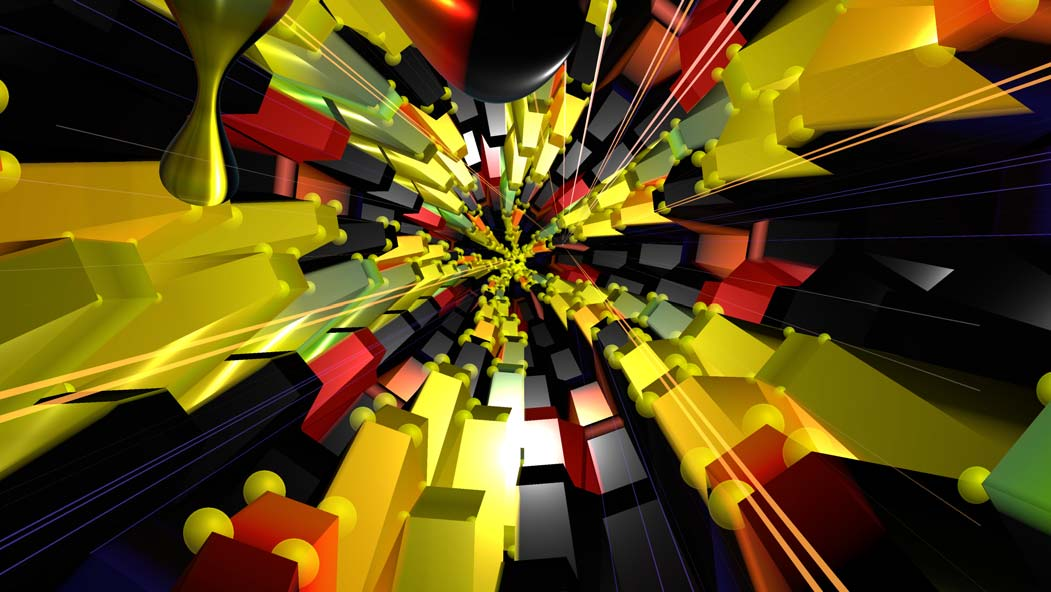
\includegraphics[width=\textwidth]{img/reused/outram2017crystal1.png}}%
    \\
    \subfloat[\centering A screenshot from the second main part of \textit{Crystal Vibes}, in which sound visualisation in the form of colour flows through an endless lattice of spheres.\crfootnote{outram2017crystal}]{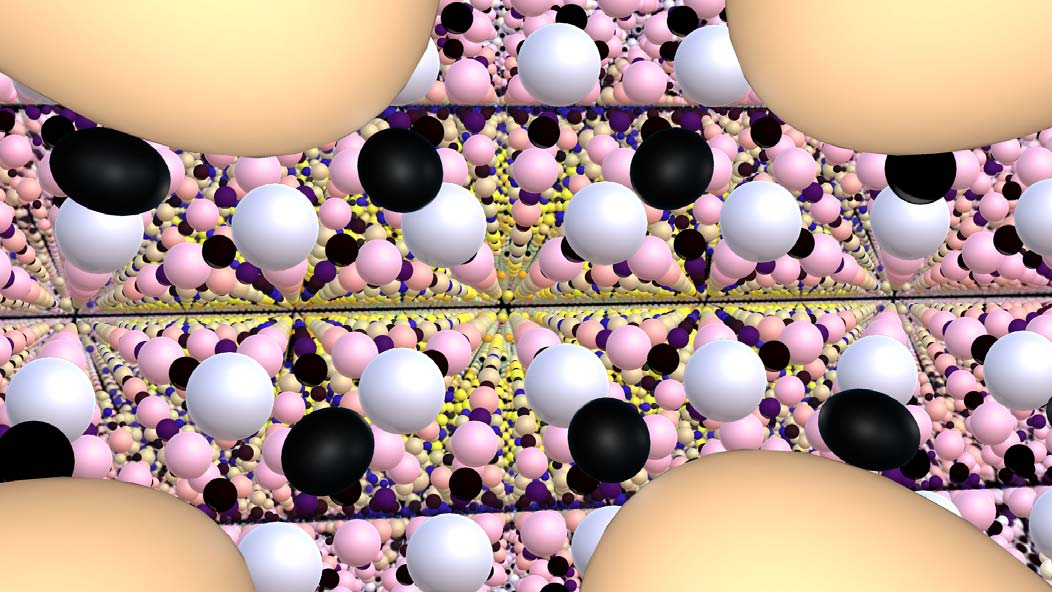
\includegraphics[width=\textwidth]{img/reused/outram2017crystal2.png}}%
    \caption{Screenshots of the \textit{Crystal Vibes} \ac{VR} application.}%
    \label{fig:outram2017crystal}%
\end{figure}

\subsubsection{Isness}
The paper \autocite{glowacki2020isness} accompanying the project \textit{Isness} proposes that so-called \acp{MTE}, that are often experienced under the influence of psychedelic drugs, may also be facilitated by virtual reality. The paper justifies this proposal by conducting a study with 57 participants analyzing participants' responses to the \ac{MEQ30}, commonly used to evaluate the effects of psychedelic drugs. The results of the study indicated that \textit{Isness} participants reported \acp{MTE} comparable to those reported in double-blind clinical studies after high doses of psilocybin and LSD.

The \ac{VR} application was designed to be used by 4 participants at a time with the \textit{HTC Vive Pro} \acp{HMD}. To provide multiplayer functionality, the client/server architecture was chosen, with each \ac{HMD} being connected to a separate \acs{GPU}-accelerated server.

The abstract virtual environments have been designed by defining a set of `aesthetic hyperparameters', each affecting a different aspect of the simulated \ac{MTE}. The overall \textit{Isness journey} was comprised of a set of states, each of which had some specific time duration. This approach allowed for reproducibility necessary for the study.

Participants were equipped with specially-made `Mudra gloves', which would create a light source within the virtual scene when they made a `mudra pose' by bringing the tip of a thumb to their forefinger or middle finger.

The entire \textit{Isness journey} was divided into 3 phases:

\begin{enumerate}
    \item Phase 1: Preparation. 15-20 minutes, included information about practical issues (phones off, toilet locations, placing posessions in a safe place), screening, description of the experience, information that the participants could withdraw at any point, and acquisition of verbal and written consent for participation in the study. This phase also included some group exercises to build rapport between participants.
    \item Phase 2: Multi-person \ac{VR} session. 35 minutes with a pre-recorded narrative soundtrack. The \ac{VR} experience was preceded by a blindfolded, narrated group meditation. Each participant was then fitted with a VR headset and the administrator initiated the \ac{VR} session, moving through 15 prespecified states, each composed from a set of aesthetic hyperparameters.
    \item Phase 3: Integration. The \acp{HMD} were taken off. Breath exercises and group exercises followed. Participants were then invited to share in a 10-15 minute facilitated discussion, after which they were provided a blank piece of paper for reflective writing, along with a blank \ac{MEQ30}.
\end{enumerate}

It is fair to say that the \textit{Isness} project focuses mainly on the replication of \acp{MTE}, whose characteristics include a sense of connectedness, transcendence, and ineffability; specifically the effects of \acp{ASC} on emotion and cognition, rather than the effects on sensory perception, as is also evident by the \ac{MEQ30} questionnaire used in the study. This can be seen in the emphasis on the narrated structure of the \textit{Isness journey}, the inclusion of a meditation session, as well as in the multiplayer design of the overall experience, that encourages interaction between participants.

That is to say, the \textit{Isness journey} has been effective in creating a memorable, subjectively meaningful experience comparable to \acp{ASC} induced by psychedelic drugs.

\begin{figure}%
    \centering
    \subfloat[\centering \textit{Isness} multi-person VR setup.\ccfootnote{glowacki2020isness}{BY-SA}{4.0}{A cropped version with label removed of}{Isness multi-person VR setup}]{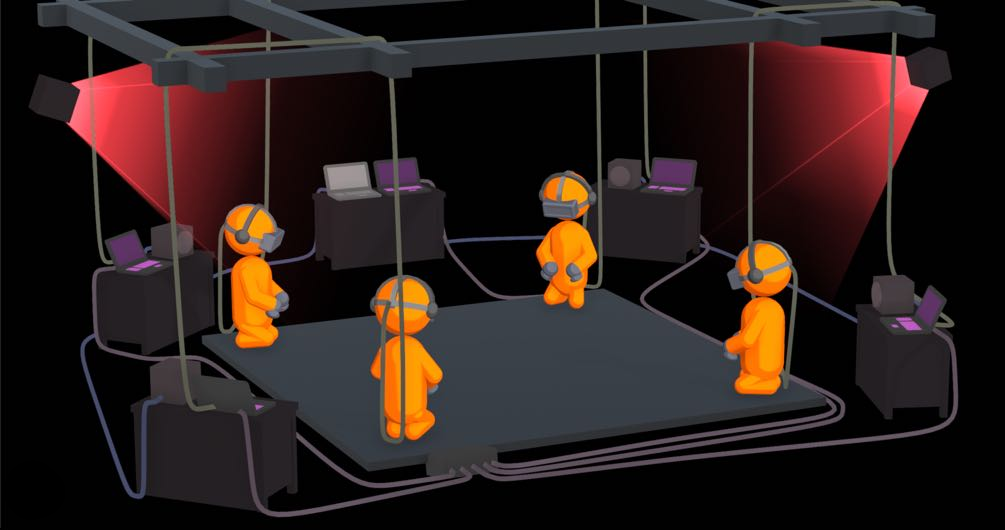
\includegraphics[width=\textwidth*\real{0.45}]{img/reused/glowacki2020isness1.png}}%
    \quad
    \subfloat[\centering In-world view of an \textit{Isness} state.\ccfootnote{glowacki2020isness}{BY-SA}{4.0}{A cropped version with label removed of}{In-world view of an Isness state}]{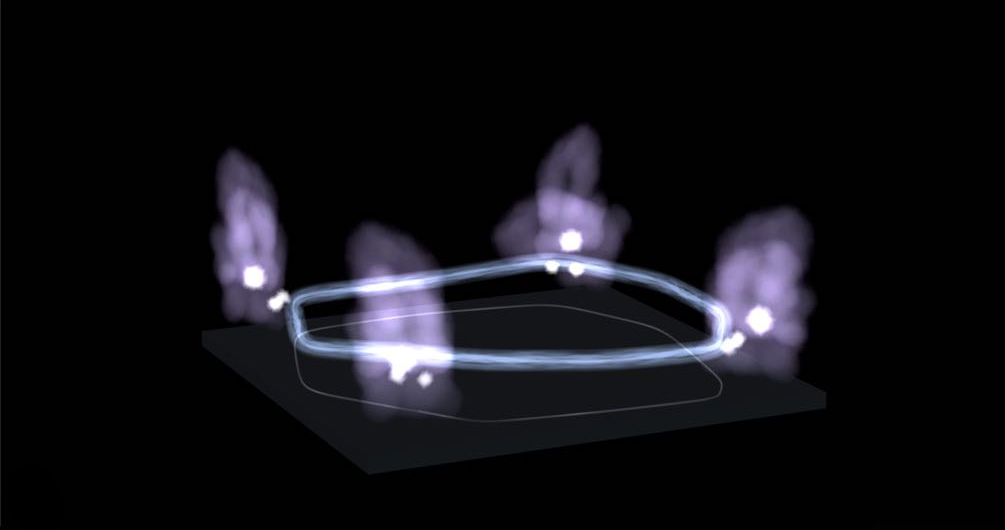
\includegraphics[width=\textwidth*\real{0.45}]{img/reused/glowacki2020isness2.png}}%
    \caption{Design of the \textit{Isness} \ac{VR} application.}%
    \label{fig:glowacki2020isness}%
\end{figure}

\subsubsection{Hallucination Machine}\label{sec:hallucination_machine}
\textit{Hallucination Machine} \autocite{suzuki2018hallucination} makes use of the \textit{DeepDream} \autocite{mordvintsev2015inceptionism} technology to alter spherical panoramic video. The altered video is then viewed through a \ac{HMD}. The usage of \textit{DeepDream} successfully simulates the sense of an increased ability to recognize patterns during certain \acp{ASC}.

While it is a compelling concept, there are many drawbacks to this approach.

\begin{enumerate}
    \item The alteration caused by \textit{DeepDream} is heavily dependent on the source data the \ac{DCNN} is trained with. If, for example, the \ac{DCNN} is trained with images of puppies, the alteration by this \ac{DCNN} will result in \textit{hallucinated} puppies.
    \item The panoramic spherical videos are not stereoscopic, hence the sense of depth is lost.
    \item Finally, the fact that the \textit{DeepDream} technology is computationally demanding may have resulted in the choice to use pre-recorded videos rather than real-time footage. This, however, limits the applications of the solution.
\end{enumerate}

However, what the \textit{DeepDream} technology does well is the simulation of the sense of an increased ability to recognize patterns, otherwise known as pareidolia, characteristic of certain \acp{ASC}. For this reason, it has found popular use in research as a way to simulate hallucinations \autocites{greco2021increased}{rastelli2021simulated}.

\begin{figure}%
    \centering
    \subfloat[\centering Original image.\cczerofootnote{Martin Thoma}]{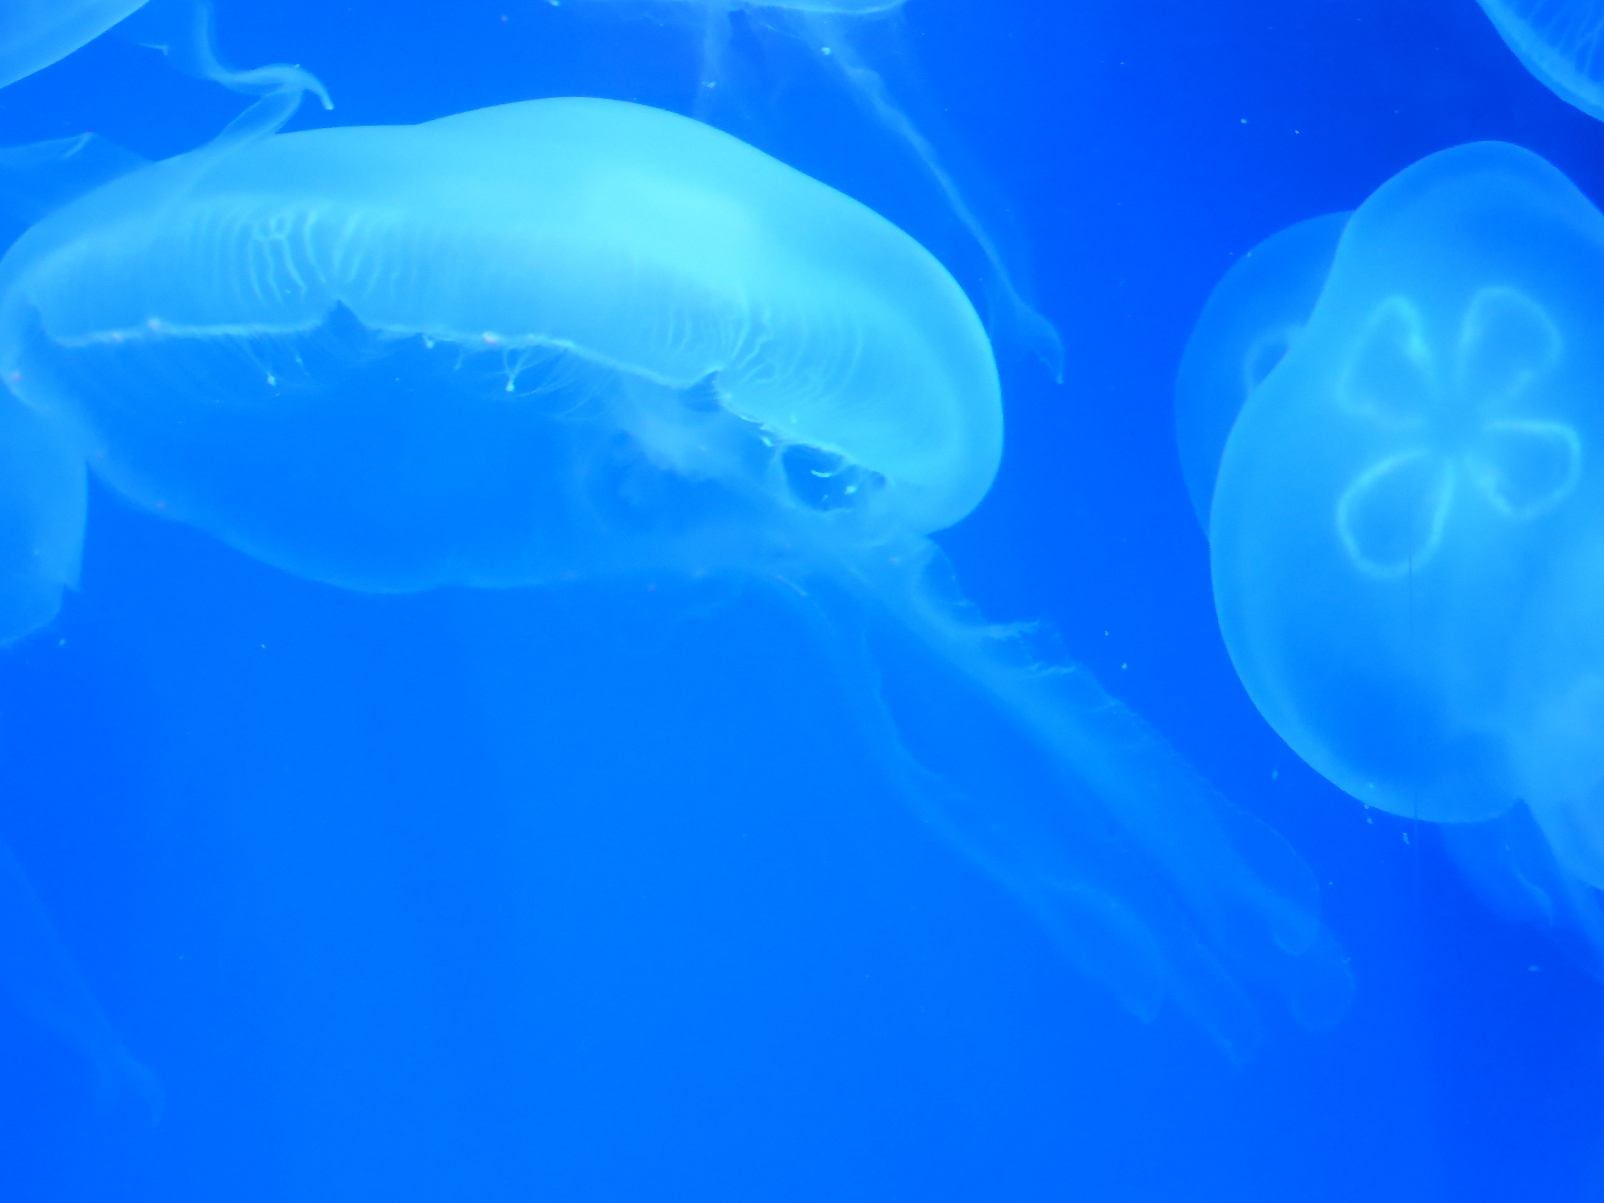
\includegraphics[width=\textwidth*\real{0.45}]{img/reused/deepdream1.jpg}}%
    \quad
    \subfloat[\centering Image altered by \textit{DeepDream}.\cczerofootnote{Martin Thoma}]{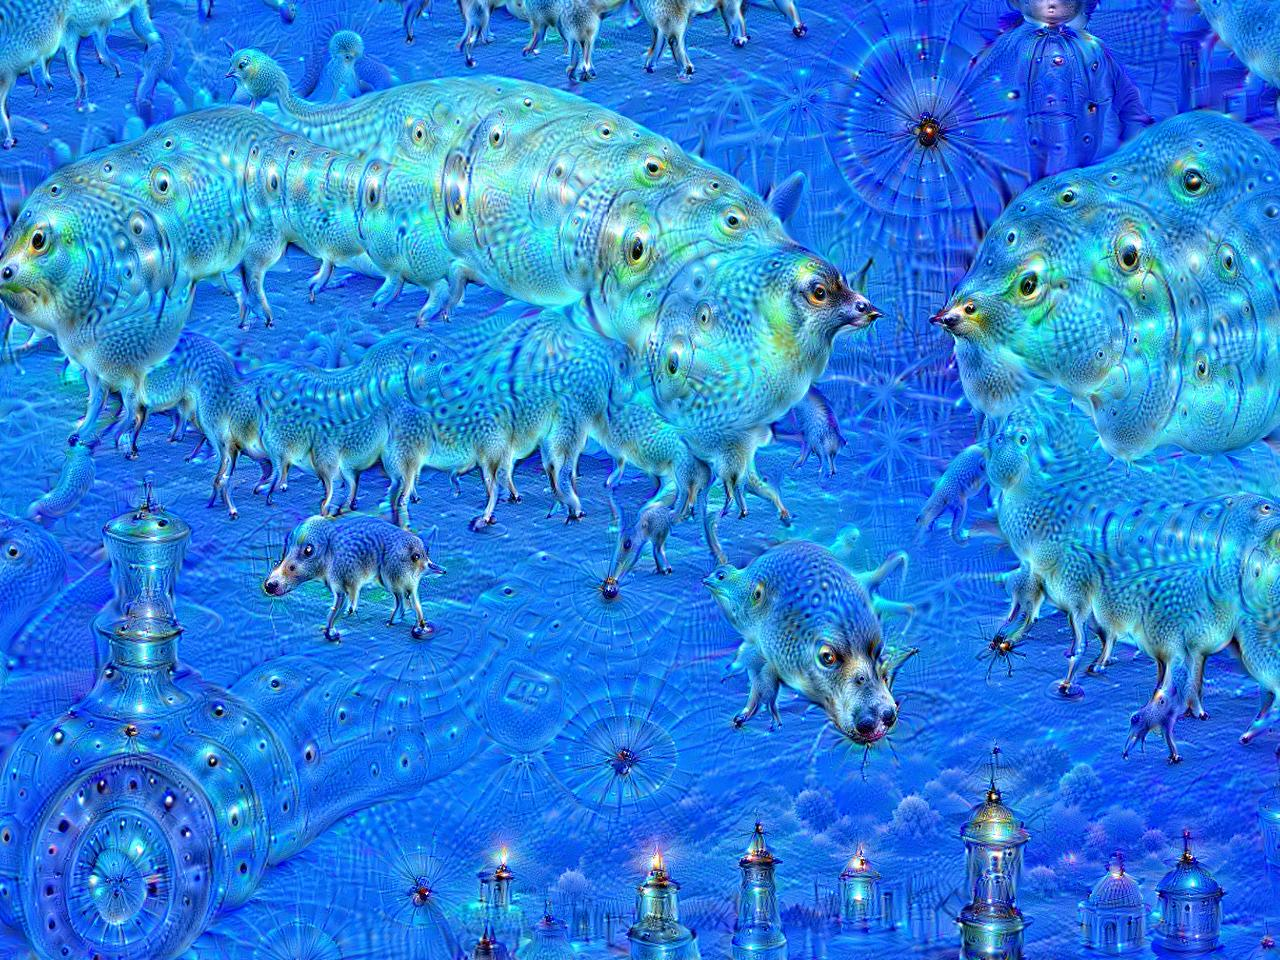
\includegraphics[width=\textwidth*\real{0.45}]{img/reused/deepdream2.jpg}}%
    \caption{Example result of applying the \textit{DeepDream} technology to an image.}%
    \label{fig:mordvintsev2015inceptionism}%
\end{figure}

\subsubsection{Lucid Loop}
\textit{Lucid Loop} \autocite{kitson2019lucid} is a proposed \ac{VR} application that makes use of an \ac{EEG} device (along with other biosensors) for biofeedback. The application is a proposed training aid for maintaining awareness during lucid dreaming, a state reached when a person becomes aware they are dreaming.

The application makes use of a \ac{HMD} to display \textit{DeepDream}-altered \autocite{mordvintsev2015inceptionism} content with the intensity of alteration corresponding to the current brain wave distribution of the wearer --- as higher frequency brain waves dominate, the displayed content becomes less affected by \textit{DeepDream}, resulting in more clarity; as lower frequency brain waves dominate, the displayed content becomes more affected and is interpreted as more dreamy and abstract.

The concept is promising, but the choice of \textit{DeepDream} might prove to be challenging to implement effectively, as the intensity of the \textit{DeepDream} alteration of displayed content is dynamic. The \textit{DeepDream} algorithm would either have to be applied in real-time, which is problematic due to the algorithm's high computational demands, or an optimization scheme would have to be used. One such optimization scheme, assuming spherical panoramic video as displayed content, might pre-render the video as altered by \textit{DeepDream} for several levels of intensity, and then during usage, would interpolate between the pre-rendered videos.

Finally, while the tool is supposed to aid in helping maintain awareness during lucid dreaming, I find it to be a missed opportunity, that the paper does not address the event that high frequency brain waves, while perhaps corresponding to greater awareness, might also cause the dreamer to wake up. A possible improvement of this tool might take this into consideration and also provide biofeedback for this event, such as fading the displayed content to white as the user becomes ``too aware''.

\subsubsection{Other AI--based Approaches}
\textcite{schartner2020neural} develop two models for generating image distortions reminiscent of verbal reports from clinical trials of \ac{DMT}.

In the first approach, the authors employed the \textit{StyleGAN} algorithm \autocite{karras2019cvpr} and modified it such that no noise input was added during the generation process, according to a hypothesized brain mechanism. This resulted in smoother, painterly look of the images.

In the second approach, the authors used the \textit{Fast Neural-Style Pytorch Implementation for Artistic Style Transfer} \autocite{johnson2016perceptual}. This method allows for the depiction of nearly any report of a visual hallucination, assuming one can find a matching content and style image.

\begin{figure}%
    \centering
    \subfloat[\centering Effect of \textit{StyleGAN} with varying levels of noise.\ccfootnote{schartner2020neural}{BY-SA}{4.0}{A cropped version of}{NVIDIA’s generative model with noise perturbation and analogous hypothesized brain mechanism}]{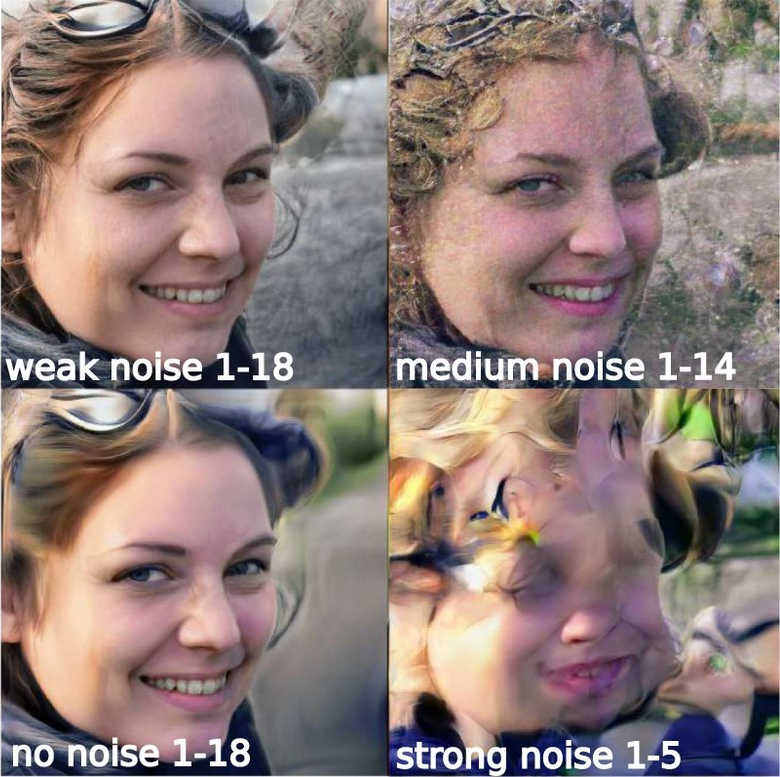
\includegraphics[height=5cm]{img/reused/schartner2020neural1.png}}%
    \qquad
    \subfloat[\centering Effect of a style transfer network with varying levels of bias.\ccfootnote{schartner2020neural}{BY-SA}{4.0}{}{Example output of a style-transfer network}]{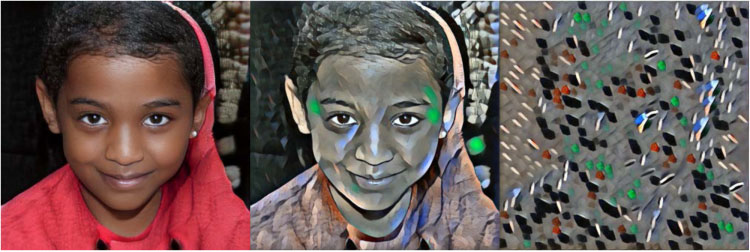
\includegraphics[height=2.5cm]{img/reused/schartner2020neural2.png}}%
    \caption{Results from the modification of \textit{StyleGAN} and the usage of a style transfer network.}%
    \label{fig:schartner2020neural}%
\end{figure}

\subsection{Tactile Stimulation Interfaces}\label{sec:tactile_stimulation_interfaces}
\ac{VR} interfaces provide a way to replace sensory information with information provided by the \ac{VR} application. Different kinds of interfaces have been developed since the conceptualization of \ac{VR}, but among the most practical and commercially available is the \ac{HMD}, which includes stereoscopic screens for visual information, and usually provides a way to substitute auditory information as well, either by providing built-in headphones or an audio connection to connect external headphones to. The main purpose of these interfaces is to provide (or improve the amount of) immersion within the virtual scene.

Among other \ac{VR} interfaces, \textit{tactile stimulation interfaces} deserve a special mention, because of their relevance to the simulation of \acp{ASC}, in particular, the simulation of haptic and auditory synasthesia, and because of their past usage in related projects. In this section, we mention several of these interfaces.

% \Needspace{200pt}
\newpage
\subsubsection{Synesthesia Suit for Rez Infinite}\label{sec:synesthesia_suit}
\begin{wrapfigure}{r}{0.45\textwidth}
    \centering
    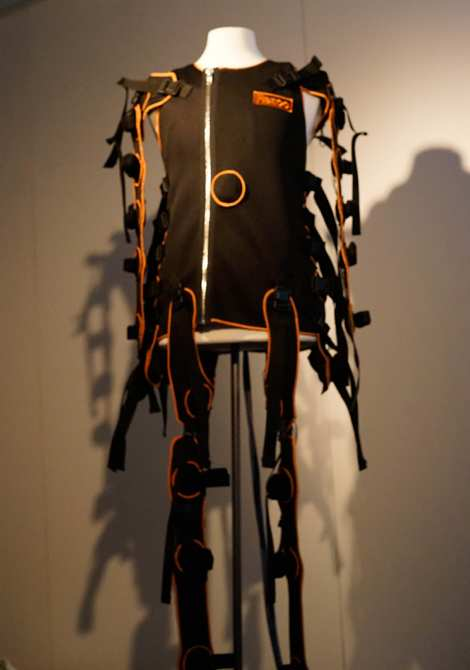
\includegraphics[width=\textwidth * \real{0.40}]{img/reused/konishi2016synesthesia.png}
    \caption{The \textit{Synesthesia Suit}.\protect\footnotemark}
\end{wrapfigure}
\footnotetext{\crtext{konishi2016synesthesia2}}

The \textit{Synesthesia Suit} \autocites{konishi2016synesthesia1}{konishi2016synesthesia2}{synesthesia2016suit} is a full-body suit that provides haptic sensation via 24 actuators, all of which can be independently controlled. The suit has been developed for the \ac{VR} game \textit{Rez Infinite} \autocite{enhance2016rezinfinite}. The aforementioned \ac{VR} game \textit{Crystal Vibes feat. Ott.} (see \ref{sec:crystal_vibes}; \textcite{outram2017crystal}) has been developed to demonstrate the capabilities of this suit.

In the game \textit{Rez Infinite}, the suit would provide feedback for interactions like shooting, hitting, and warping. The suit would respond to collisions in the virtual world, as well as to the in-game action and sounds.

The design of the \textit{Synesthesia Suit} was later improved by \textit{Synesthesia Wear} \autocite{furukawa2019synesthesia}, which adds wireless connections and improves user intuitiveness and customizability in the placement of the actuators.

\subsubsection{Synesthesia X1 - 2.44}
\textit{Synesthesia X1 - 2.44} \autocite{synesthesia2021x1} is a seat with 2 speakers and 44 vibrotactile actuators. While it has been presented without a \ac{HMD}, the possibility of using a \ac{HMD} while seated is available, but the design of this tactile interface as a seat makes it impossible for the user to move around. Still, it might be suitable used for the development of a more passive \ac{VR} experience.

\subsubsection{Subpac}
Commercial wearable subwoofers, such as the \textit{Subpac} \autocite{subpac2013subpac}, are able to have a significant impact on immersion \autocite{drempetic2017wearable} even for non-\ac{VR} content.

The \textit{Subpac} has been used in \textit{Longing for Wilderness} \autocite{zimmermann2016longing}, a \ac{VR} experience that ``takes you from the noisy city through the slowly transforming forest towards a calm and airy landscape''. The sound design of the application has been specially made with the device in mind.

\section{Contributions}
We develop a \ac{VR} application for \acp{HMD} that simulates select aspects of \acp{ASC}.
We perform a study in which we measure the influence of the created \ac{VR} application on the human mind. This measurement is done via the \ace{11-ASC}{\textcite{studerus2010psychometric}}, that is used in clinical studies of psychedelic drugs.
